% TO DO:
% 5.2.2) Update maxout formula
% 5.2.3) Update loss functions for Absolute and Huber in Table 2
% 5.2.3) Starting with this section, use algorithm mode to outline algos like SGD
% Appendix parameters:  Add notes on acceptable ranges.  ie.  rho in [0,1]?
% Are there any parameters that should be marked as Optional or Experimental?


% NOTES:
% Some of the parameter definitions in the appendix have R-specific flavor to them.  For example, c(100,100) is specific to R.
% Some of the parameters listed here are not available in R (and probably Python).  For example, _target_ratio_comm_to_comp
% Some references are in parenthesis and some are not.... need to standardize citations in text
% A few of the arguments are deprecated (according to Arno), but they still appear in the code, so I don't know if we should include them or not in our arg list.  Right now they appear as "(Deprecated)" below
% On the arglist, what does Optional indicate?  Many are not marked as optional... but are actually Optional.  Not sure (Optional) is being used properly.
% Many of the params in the arglist are shared with other algos, let's make sure those definitions are identical between booklets.
% Maybe move the Load Data section to the Use Case section (like GBM)

\documentclass[a4paper, twoside]{article}
\setcounter{secnumdepth}{5}
\setcounter{tocdepth}{5}
\usepackage[english]{babel}
\usepackage{textcomp}
\usepackage{amsmath,amsthm,amsfonts,amssymb,epsfig}
\usepackage{array}
\usepackage{datetime}
\usepackage{lipsum}% http://ctan.org/pkg/lipsum
\usepackage[left=1.1in,top=1in,right=1.1in]{geometry}% http://ctan.org/pkg/geometry
\usepackage{listings}% http://ctan.org/pkg/listings
\usepackage{spverbatim}
\usepackage{hyperref}
\usepackage{microtype}
\hypersetup{colorlinks=true, urlcolor=black, linkcolor=black}
\usepackage{graphicx}
\graphicspath{ {images/} }
\usepackage{parskip}
\usepackage{titlesec} %used for diminishing heading sizes
\usepackage[square, sort, comma, numbers]{natbib} %%uses titles for cited references
\usepackage[fit]{truncate}
\usepackage{fancyhdr}
\pagestyle{fancy}
\fancyhead{}
\fancyhead[RO, RE]{\thepage}
\fancyhead[LO, LE]{\rightmark}
\renewcommand{\sectionmark}[1]{\markboth{}{\textsc{\thesection~#1}}}
\fancyfoot[C]{}%hide footer
\usepackage{xcolor} 
\usepackage[scaled=1]{couriers}

\xdefinecolor{gray}{rgb}{0.6,0.6,0.6} 


\titleformat*{\section}{\LARGE\bfseries\sffamily}
\titleformat*{\subsection}{\Large\bfseries\sffamily}
\titleformat*{\subsubsection}{\large\bfseries\sffamily}
\titleformat*{\paragraph}{\large\bfseries\sffamily}
\titleformat*{\subparagraph}{\large\bfseries\sffamily}
\renewcommand{\familydefault}{\sfdefault} %sans-serif font





\begin{document}

%----------------------------------------------------------------------
% Definition for "lstlisting" blocks
%----------------------------------------------------------------------
% --- USAGE ---
%
% \begin{lstlisting}[style=R}
% ...
% \end{lstlisting}
%
% % \begin{lstlisting}[style=output}
% ...
% \end{lstlisting}
%----------------------------------------------------------------------

% By default, make listings all black so it's easy to spot the ones that aren't set to a style.
% This is just a debugging technique.
\lstset{backgroundcolor=\color{black}}

% Define scala language first
% ``define'' Scala
\lstdefinelanguage{scala}{
  morekeywords={abstract,case,catch,class,def,%
    do,else,extends,false,final,finally,%
    for,if,implicit,import,match,mixin,%
    new,null,object,override,package,%
    private,protected,requires,return,sealed,%
    super,this,throw,trait,true,try,%
    type,val,var,while,with,yield},
  otherkeywords={=>,<-,<\%,<:,>:,\#,@},
  sensitive=true,
  morecomment=[l]{//},
  morecomment=[n]{/*}{*/},
  morestring=[b]``,
  morestring=[b]',
  morestring=[b]''``
}

\lstdefinestyle{R}{
  language=R,
  frame=single,
  breaklines,
  basicstyle=\ttfamily,
  commentstyle=\textbf,% comment style
  keywordstyle=\ttfamily,
  numbers=left,% display line numbers on the left side 
  numberstyle=\scriptsize,% use small line numbers 
  numbersep=10pt,% space between line numbers and code
  backgroundcolor=\color{white}, 
  showstringspaces=false % don't show spaces as weird char.
}

\lstdefinestyle{python}{
  language=python,
  frame=single,
  breaklines,
  basicstyle=\ttfamily,
  commentstyle=\textsl,% comment style
  keywordstyle=\ttfamily,
  numbers=left,% display line numbers on the left side 
  numberstyle=\scriptsize,% use small line numbers 
  numbersep=10pt,% space between line numbers and code
  backgroundcolor=\color{white}, 
  showstringspaces=false %don't show spaces as weird char.
}

\lstdefinestyle{Scala}{
  language=scala,
  frame=single,
  breaklines,
  basicstyle=\ttfamily,
  commentstyle=\textsl,% comment style
  keywordstyle=\ttfamily,
  numbers=left,% display line numbers on the left side 
  numberstyle=\scriptsize,% use small line numbers 
  numbersep=10pt,% space between line numbers and code
  backgroundcolor=\color{white}, 
  showstringspaces=false % don't show spaces as weird char.
}

\lstdefinestyle{Bash}{
  language=bash,
  frame=single,
  breaklines,
  basicstyle=\ttfamily,
  commentstyle=\textsl,% comment style
  keywordstyle=\ttfamily,
  numbers=left,% display line numbers on the left side 
  numberstyle=\scriptsize,% use small line numbers 
  numbersep=10pt,% space between line numbers and code
  backgroundcolor=\color{white}, 
  showstringspaces=false % don't show spaces as weird char.
}


\definecolor{mygray}{rgb}{0.92,0.92,0.92}

\lstdefinestyle{output}{
  frame=single,
  breaklines,
  basicstyle=\ttfamily,
  numbers=left,% display line numbers on the left side 
  numberstyle=\scriptsize,% use small line numbers 
  numbersep=10pt,% space between line numbers and code
  backgroundcolor=\color{mygray}, 
  showstringspaces=false %don't show spaces as weird char.
}

\newcommand{\waterExampleInR} {
\textbf{Example in R} \\
}

\newcommand{\waterExampleInPython} {
\textbf{Example in Python} \\
}


\thispagestyle{empty} %removes page number  

\begin{center}
\textsc{\Large\bf{Deep Learning with H2O}}


\bigskip
\textsc{\small{Arno Candel \hspace{40pt} Jessica Lanford \hspace{40pt} Erin LeDell \hspace{40pt} Viraj Parmar \hspace{40pt} } }
\\
\bigskip
\line(1,0){250}  %inserts  horizontal line

{\url{http://h2o.gitbooks.io/deep-learning/}}


\bigskip
August 2015: Third Edition 
\\%add front page image here? (wavy lines)
\bigskip
\end{center}

{\raggedright\vfill\ 

Deep Learning with H2O\\
  by Arno Candel, Jessica Lanford, Erin LeDell \&\ Viraj Parmar\\
\bigskip
  Published by H2O.ai, Inc. \\
2307 Leghorn St. \\
Mountain View, CA 94043\\
\bigskip
\textcopyright 2015 H2O.ai, Inc. All Rights Reserved. 
\bigskip

August 2015: Third Edition
\bigskip

Photos by \textcopyright H2O.ai, Inc. 
\bigskip

While every precaution has been taken in the\\
preparation of this book, the publisher and\\
authors assume no responsibility for errors or\\
omissions, or for damages resulting from the\\
use of the information contained herein.\\
\bigskip
Printed in the United States of America. 
}

\newpage

\tableofcontents

%----------------------------------------------------------------------
%----------------------------------------------------------------------

\newpage

\section{Introduction}
This document introduces the reader to Deep Learning with H2O.  Examples are written in R and Python.
The reader is walked through the installation of H2O, basic deep learning concepts, building deep neural nets in H2O, how to interpret model output, how to make predictions, and various implementation details.

%----------------------------------------------------------------------
%----------------------------------------------------------------------

\section{What is H2O?}
\Urlmuskip=0mu plus 1mu\relax %needed to make long URLs break nicely


H2O is fast, scalable, open-source machine learning and deep learning for smarter applications. With H2O, enterprises like PayPal, Nielsen Catalina, Cisco, and others can use all their data without sampling to get accurate predictions faster. Advanced algorithms such as deep learning, boosting, and bagging ensembles are built-in to help application designers create smarter applications through elegant APIs. Some of our initial customers have built powerful domain-specific predictive engines for recommendations, customer churn, propensity to buy, dynamic pricing, and fraud detection for the insurance, healthcare, telecommunications, ad tech, retail, and payment systems industries.

Using in-memory compression, H2O handles billions of data rows in-memory, even with a small cluster. To make it easier for non-engineers to create complete analytic workflows, H2O's platform includes interfaces for R, Python, Scala, Java, JSON, and CoffeeScript/JavaScript, as well as a built-in  web interface, Flow. H2O was built alongside (and on top of) Hadoop and Spark Clusters and typically deploys within minutes.

H2O includes many common machine learning algorithms, such as generalized linear modeling (linear regression, logistic regression, etc.), Na\"{i}ve Bayes, principal components analysis, time series, k-means clustering, and others. H2O also implements best-in-class algorithms at scale, such as distributed random forest, gradient boosting and deep learning. Customers can build thousands of models and compare the results to get the best predictions.

H2O is nurturing a grassroots movement of physicists, mathematicians, and computer scientists to herald the new wave of discovery with data science by collaborating closely with academic researchers and Industrial data scientists. Stanford university giants Stephen Boyd, Trevor Hastie, Rob Tibshirani advise the H2O team on building scalable machine learning algorithms. With hundreds of meetups over the past three years, H2O has become a word-of-mouth phenomenon, growing amongst the data community by a hundred-fold, and is now used by 30,000+ users and is deployed using R, Python, Hadoop, and Spark in 2000+ corporations.

\textbf{Try it out}

\begin{itemize}
\item  Download H2O directly at \mbox{\url{http://h2o.ai/download}}.
\item Install H2O's R package from CRAN at {\url{https://cran.r-project.org/web/packages/h2o/}}. 
\item Install the Python package from PyPI at {\url{https://pypi.python.org/pypi/h2o/}}.

\end{itemize}



\textbf{Join the community}
\begin{itemize}
\item  To learn about our meetups, training sessions, hackathons, and product updates, visit {\url{http://h2o.ai}}. 
\item Visit the open source community forum at {\url{https://groups.google.com/d/forum/h2ostream}}.
\item Join the chat at {\url{https://gitter.im/h2oai/h2o-3}}.
\end{itemize}





%----------------------------------------------------------------------
%----------------------------------------------------------------------

\newpage

\newcommand{\waterVersion}{3.0.1.4}
\section{Installation} 
\Urlmuskip=0mu plus 1mu\relax %needed to make long URLs break nicely


The easiest way to directly install H2O is  via an R or Python package.

({\bf{Note}}: The examples in this document were created with H2O version \waterVersion.)

\subsection{Installation in R}

To load a recent H2O package from CRAN, run:

\begin{lstlisting}[style=R]
install.packages("h2o")
\end{lstlisting}

{\bf{Note}}: The version of H2O in CRAN is often one release behind the current version.

For the latest recommended version, download the
latest stable H2O-3 build from the H2O download page:

\begin{enumerate}
\item Go to {\url{http://h2o.ai/download}}.
\item Choose the latest stable H2O-3 build.
\item Click the ``Install in R'' tab.
\item Copy and paste the commands into your R session.
\end{enumerate}

\bigskip
After H2O is installed on your system, verify the installation:

\begin{lstlisting}[style=R]
library(h2o)

#Start H2O on your local machine using all available cores.
#By default, CRAN policies limit use to only 2 cores.
h2o.init(nthreads = -1)

#Get help
?h2o.glm
?h2o.gbm

#Show a demo
demo(h2o.glm)
demo(h2o.gbm)
\end{lstlisting}

\subsection{Installation in Python}

To load a recent H2O package from PyPI, run:

\begin{lstlisting}[style=python]
pip install h2o
\end{lstlisting}

To download the
latest stable H2O-3 build from the H2O download page:

\begin{enumerate}
\item Go to {\url{http://h2o.ai/download}}.
\item Choose the latest stable H2O-3 build.
\item Click the ``Install in Python'' tab.
\item Copy and paste the commands into your Python session.
\end{enumerate}

\bigskip
After H2O is installed, verify the installation:

\begin{lstlisting}[style=python]
import h2o

# Start H2O on your local machine
h2o.init()

# Get help
help(h2o.glm)
help(h2o.gbm)

# Show a demo
h2o.demo("glm")
h2o.demo("gbm")

\end{lstlisting}

\subsection{Pointing to a Different H2O Cluster}

The instructions in the previous sections create a one-node H2O cluster on your local machine. 

To connect to an established H2O cluster (in a multi-node Hadoop environment, for example) specify the IP address and port number for the established cluster using the \texttt{ip} and \texttt{port} parameters in the \texttt{h2o.init()} command.  The syntax for this function is identical for R and Python:
\medskip  

\begin{lstlisting}[style=R]
h2o.init(ip = "123.45.67.89", port = 54321)
\end{lstlisting}

%if it's the same, only one is needed



\subsection{Example code}

R code for the examples in this document are available here:

\url{https://github.com/h2oai/h2o-3/blob/master/h2o-docs/src/booklets/v2_2015/source/DeepLearning_Vignette.R}

Python code for the examples in this document can be found here:

\url{https://github.com/h2oai/h2o-3/blob/master/h2o-docs/src/booklets/v2_2015/source/DeepLearning_Vignette.ipynb}

The document source itself can be found here:

\url{https://github.com/h2oai/h2o-3/blob/master/h2o-docs/src/booklets/v2_2015/source/DeepLearning_Vignette.tex}


\newpage
\section{Deep Learning Overview}
%Deep Learning has been dominating recent machine learning competitions with better predictions. 
Unlike the neural networks of the past, modern Deep Learning has cracked the code for training stability and generalization and scales on big data.  It is often the algorithm of choice for highest predictive accuracy, as deep learning algorithms performs quite well in a number of diverse problems. 

First, we present a brief overview of deep neural networks for supervised learning tasks. There are several theoretical frameworks for deep learning, and here we summarize the feedforward architecture used by H2O. 
\\
\begin{figure}[h]
\centering
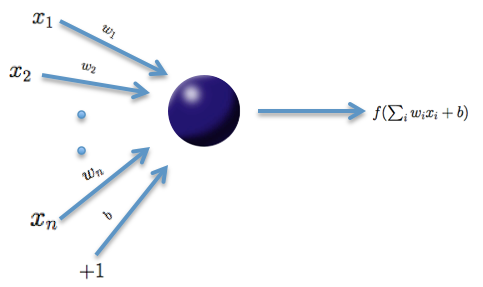
\includegraphics[scale=0.5]{neuron.png}
\end{figure}
\\
\noindent
The basic unit in the model (shown above) is the neuron, a biologically inspired model of the human neuron. For humans, varying strengths of neurons' output signals travel along the synaptic junctions and are then aggregated  as input for a connected neuron's activation. In the model, the weighted combination $\alpha = \sum_{i=1}^{n} w_i x_i + b$ of input signals is aggregated, and then an output signal $f(\alpha)$ transmitted by the connected neuron. The function $f$ represents the nonlinear activation function used throughout the network, and the bias $b$ accounts for the neuron's activation threshold.
\\
\begin{figure}[h!]
\centering
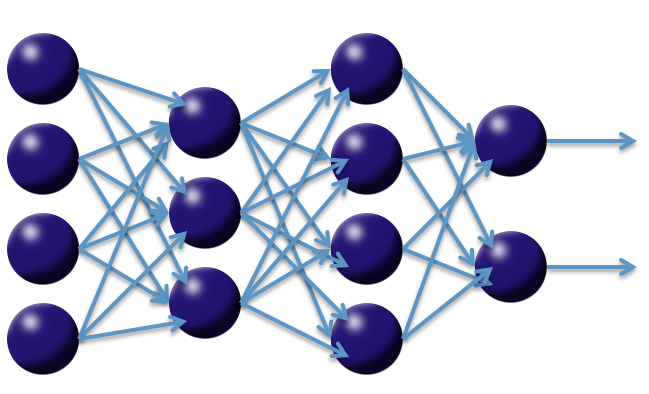
\includegraphics[scale=0.3]{net.png}
\end{figure}
\\
\noindent
Multi-layer, feedforward neural networks consist of many layers of interconnected neuron units, starting with an input layer to match the feature space, followed by multiple layers of nonlinearity, and ending with a linear regression or classification layer to match the output space. The inputs and outputs of the model's units follow the basic logic of the single neuron described above. Bias units are included in each non-output layer of the network. The weights linking neurons and biases with other neurons fully determine the output of the entire network, and learning occurs when these weights are adapted to minimize the error on labeled training data. More specifically, for each training example $j$, the objective is to minimize a loss function, 
\begin{center}
$L(W,B$ $|$ $j)$.
\end{center}
Here, $W$ is the collection $\left\{W_i\right\}_{1:N-1}$, where $W_i$ denotes the weight matrix connecting layers $i$ and $i+1$ for a network of $N$ layers. Similarly $B$ is the collection $\left\{b_i\right\}_{1:N-1}$, where $b_i$ denotes the column vector of biases for layer $i+1$.
This basic framework of multi-layer neural networks can be used to accomplish deep learning tasks. Deep learning architectures are models of hierarchical feature extraction, typically involving multiple levels of nonlinearity. Deep learning models are able to learn useful representations of raw data and have exhibited high performance on complex data such as images, speech, and text \href{http://www.iro.umontreal.ca/~lisa/pointeurs/TR1312.pdf}{(Bengio, 2009)}. 


\section{H2O's Deep Learning architecture} 

As described above, H2O follows the model of multi-layer, feedforward neural networks for predictive modeling. This section provides a more detailed description of H2O's Deep Learning features, parameter configurations, and computational implementation.

\subsection{Summary of features} 
H2O's Deep Learning functionalities include:

\begin{itemize}

\item purely supervised training protocol for regression and classification tasks

\item fast and memory-efficient Java implementations based on columnar compression and fine-grain Map/Reduce

\item multi-threaded and distributed parallel computation to be run on either a single node or a multi-node cluster

\item fully automatic per-neuron adaptive learning rate for fast convergence

\item optional specification of learning rate, annealing and momentum options

\item regularization options include L1, L2, dropout, Hogwild! and model averaging to prevent model overfitting

\item elegant web interface or fully scriptable R API from H2O CRAN package

\item grid search for hyperparameter optimization and model selection

\item model checkpointing for reduced run times and model tuning

\item automatic data pre and post-processing for categorical and numerical data

\item automatic imputation of missing values

\item automatic tuning of communication vs computation for best performance  %assuming this is a reference to the force_load_balance param?

\item model export in plain java code for deployment in production environments

\item additional expert parameters for model tuning

\item deep autoencoders for unsupervised feature learning and anomaly detection capabilities

\end{itemize}


\subsection{Training protocol} 
The training protocol described below follows many of the ideas and advances in the recent deep learning literature.

\subsubsection{Initialization}
\label{sssec:Initialization}
\noindent
Various deep learning architectures employ a combination of unsupervised pretraining followed by supervised training, but H2O uses a purely supervised training protocol. The default initialization scheme is the uniform adaptive option, which is an optimized initialization based on the size of the network. Alternatively, you may select a random initialization to be drawn from either a uniform or normal distribution, for which a scaling parameter may be specified as well.
\subsubsection{Activation and loss functions} \label{sssec:ActivationLoss}
In the introduction, we described the nonlinear activation function $f$; the choices are summarized in Table 1. Note here that $x_i$ and $w_i$ denote the firing neuron's input values and their weights, respectively; $\alpha$ denotes the weighted combination $\alpha = \sum_i w_i x_i+b$.
\begin{table}[ht] 
\caption{Activation functions }
% title of Table 
\centering % used for centering table 
\begin{tabular}{c c c} % centered columns (4 columns) 
\hline\hline %inserts double horizontal lines 
Function & Formula & Range \\ [0.5ex] % inserts table 
%heading 
\hline % inserts single horizontal line 
Tanh & $f(\alpha) = \frac{e^{\alpha} - e ^{-\alpha}}{e^\alpha + e ^{-\alpha}}$ & $f(\cdot) \in [-1,1]$ \\ % inserting body of the table 
Rectified Linear & $f(\alpha) = \max(0,\alpha)$ & $f(\cdot) \in \mathbb{R}_+$ \\
Maxout & $f(\cdot) = \max(w_i x_i + b) \text{, rescale if} \max f(\cdot) \geq 1 $ & $f(\cdot) \in [-\infty,1]$\\  % [1ex] adds vertical space
\hline %inserts single line 
\end{tabular} 
\label{table:nonlin} % is used to refer this table in the text 
\end{table}
The $\tanh$ function is a rescaled and shifted logistic function and its symmetry around 0 allows the training algorithm to converge faster. The rectified linear activation function has demonstrated high performance on image recognition tasks, and is a more biologically accurate model of neuron activations (\href{http://yann.lecun.com/exdb/publis/pdf/lecun-98b.pdf}{LeCun et al, 1998}).  Maxout activation works particularly well with dropout, a regularization method discussed later in this vignette (\href{http://arxiv.org/pdf/1302.4389.pdf}{Goodfellow et al, 2013}). 
It is difficult to determine a ``best" activation function to use; each may outperform the others in separate scenarios, but grid search models (also described later) can help to compare activation functions and other parameters. The default activation function is the Rectifier. Each of these activation functions can be operated with dropout regularization (see below).

The following choices for the loss function $L(W,B$ $|$ $ j)$ are summarized in Table 2. The system default enforces the table's typical use rule based on whether regression or classification is being performed. Note here that $t^{(j)}$ and $o^{(j)}$ are the predicted (target) output and actual output, respectively, for training example $j$; further, let $y$ denote the output units and $O$ the output layer.
\\
% TO DO: Update loss functions for Absolute and Huber
\begin{table}[ht] 
\caption{Loss functions }
% title of Table 
\centering % used for centering table 
\begin{tabular}{c c c} % centered columns (4 columns) 
\hline\hline %inserts double horizontal lines 
Function & Formula & Typical use \\ [0.5ex] % inserts table 
%heading 
\hline % inserts single horizontal line 
Mean Squared Error & $L(W,B | j) = \frac{1}{2}\|t^{(j)} - o^{(j)}\|_2^2$ & Regression \\ % inserting body of the table 
Absolute & $L(W,B | j)$ = TO DO & Regression \\
Huber & $L(W,B | j)$ = TO DO & Regression \\
Cross Entropy & $L(W,B | j) = -\sum\limits_{y \in O} \left(\ln(o_y^{(j)}) \cdot t_y^{(j)} + \ln(1-o_y^{(j)}) \cdot (1-t_y^{(j)})\right) $ & Classification \\
\hline %inserts single line 
\end{tabular} 
\label{table:nonlin} % is used to refer this table in the text 
\end{table}

\subsubsection{Parallel distributed network training} 

The procedure to minimize the loss function $L(W,B$ $|$ $j)$ is a parallelized version of stochastic gradient descent (SGD). Standard SGD can be summarized as follows, with the gradient $\nabla L(W,B$ $|$ $j)$ computed via backpropagation (\href{http://yann.lecun.com/exdb/publis/pdf/lecun-98b.pdf}{LeCun et al, 1998}). The constant $\alpha$ indicates the learning rate, which controls the step sizes during gradient descent.
\\
\\
{\bf{\footnotesize{Standard stochastic gradient descent}}}
\\
\line(1,0){275}
\\
1. Initialize $W,B$ 
\\
2. Iterate until convergence criterion reached:

\hspace{1cm} a. Get training example $i$

\hspace{1cm} b. Update all weights $w_{jk} \in W$, biases $b_{jk} \in B$

\hspace{2cm}  $w_{jk} := w_{jk} - \alpha \frac{\partial L(W,B | j)}{\partial w_{jk}}$

\hspace{2cm} $b_{jk} := b_{jk} - \alpha \frac{\partial L(W,B | j)}{\partial b_{jk}}$

\line(1,0){275}
\\
\\  
Stochastic gradient descent is known to be fast and memory-efficient, but not easily parallelizable without becoming slow. We utilize \textsc{Hogwild!}, the recently developed lock-free parallelization scheme from \href{http://i.stanford.edu/hazy/papers/hogwild-nips.pdf}{Niu et al, 2011}, to address this issue. \textsc{Hogwild!} follows a shared memory model where multiple cores  (each handling separate subsets or all of the training data) are able to make independent contributions to the gradient updates $\nabla L(W,B$ $ |$ $j)$ asynchronously. In a multi-node system, this parallelization scheme works on top of H2O's distributed setup where the training data is distributed across the cluster. Each node operates in parallel on its local data until the final parameters $W,B$ are obtained by averaging. Below is a rough summary.
\\
\\
\noindent
{\bf{\footnotesize{Parallel distributed and multi-threaded training with SGD in H2O Deep Learning}}}
\\
\line(1,0){440}
\\
1. Initialize global model parameters $W,B$
\\
2. Distribute training data $\mathcal{T}$ across nodes (can be disjoint or replicated)
\\
3. Iterate until convergence criterion reached:

\hspace{1cm} 3.1. For nodes $n$ with training subset $\mathcal{T}_n$, do in parallel:

\hspace{2cm}  a. Obtain copy of the global model parameters $W_n, B_n$

\hspace{2cm}  b. Select active subset $\mathcal{T}_{na} \subset \mathcal{T}_n$ (user-given number of samples per iteration)

\hspace{2cm}  c. Partition $\mathcal{T}_{na}$ into $\mathcal{T}_{nac}$ by cores $n_c$

\hspace{2cm}  d. For cores $n_c$ on node $n$, do in parallel:

\hspace{3cm}  i. Get training example $i \in \mathcal{T}_{nac}$

\hspace{3cm}  ii. Update all weights $w_{jk} \in W_n$, biases $b_{jk} \in B_n$

\hspace{4cm}  $w_{jk} := w_{jk} - \alpha \frac{\partial L(W,B | j)}{\partial w_{jk}}$

\hspace{4cm} $b_{jk} := b_{jk} - \alpha \frac{\partial L(W,B | j)}{\partial b_{jk}}$

\hspace{1cm} 3.2. Set $W,B := $ Avg$_n$ $W_n,$ $ $Avg$_n$ $B_n$

\hspace{1cm} 3.3. Optionally score the model on (potentially sampled) train/validation scoring sets
\\
\line(1,0){440}
\\
\\
Here, the weights and bias updates follow the asynchronous  $\textsc{Hogwild!}$ procedure to incrementally adjust each node's parameters $W_n,B_n$ after seeing example $i$. The Avg$_n$ notation refers to the final averaging of these local parameters across all nodes to obtain the global model parameters and complete training.

\subsubsection{Specifying the number of training samples per iteration} 
\label{sssec:TrainSamplesPerIter}
H2O Deep Learning is scalable and can take advantage of large clusters of compute nodes. There are three operating modes. The default behavior is to let every node train on the entire (replicated) dataset, but automatically  shuffling (and/or using a subset of) the training examples for each iteration locally. For datasets that don't fit into each node's memory (depending on the amount of heap memory specified by the \texttt{-XmX} Java %(or \texttt{max\_mem\_size} in R) 
option), it might not be possible to replicate the data, and each compute node can be instructed to train only with local data. An experimental single node mode is available for cases where final convergence is slow due to the presence of too many nodes, but this has not been necessary in our testing.

The number of training examples globally presented to the distributed SGD worker nodes between model averaging is defined by the parameter \texttt{train\_samples\_per\_iteration}. If the specified value is \texttt{-1}, all nodes process all their local training data per iteration. If \texttt{replicate\_training\_data} is enabled, which is the default setting, this will result in training N epochs (passes over the data) per iteration on N nodes; otherwise, one epoch will be trained per iteration. Another special value is \texttt{0}, which always results in one epoch per iteration, regardless of the number of compute nodes. In general, any user-specified positive number is permissible for this parameter. For large datasets, we recommend specifying a fraction of the dataset. 

For example, if the training data contains $10$ million rows, and we specify the number of training samples per iteration as $100,000$ when running on four nodes, then each node will process $25,000$ examples per iteration, and it will take $40$ distributed iterations to process one epoch. If the value is too high, it might take too long between synchronization and model convergence may be slow.  If the value is too low, network communication overhead will dominate the runtime and computational performance will suffer. A value of \texttt{-2}, which is the default value, enables auto-tuning for this parameter, based on the computational performance of the processors and the network of the system, and attempts to find a good balance between computation and communication. This parameter can affect the convergence rate during training.
\\
\noindent
\subsection{Regularization} 
\label{ssec:Regularization}
H2O's Deep Learning framework supports regularization techniques to prevent overfitting. 
\\
\\
$\ell_1$ (Lasso) and $\ell_2$ (Ridge) regularization enforce the same penalties as they do with other models; that is, modifying the loss function so as to minimize some loss, %%incomplete sentence? or referring to the equation below? should specify what is minimized (loss?)
\\
\begin{center}
$L'(W,B$ $|$ $j) = L(W,B$ $|$ $j) + \lambda_1 R_1(W,B$ $|$ $j) + \lambda_2 R_2(W,B$ $|$ $j)$.
\end{center}

For $\ell_1$ regularization, $R_1(W,B$ $|$ $j)$ represents of the sum of all $\ell_1$ norms of the weights and biases in the network; $R_2(W,B$ $|$ $j)$ represents the sum of squares of all the weights and biases in the network. The constants $\lambda_1$ and $\lambda_2$ are generally specified as very small, for example $10^{-5}$.
\\

The second type of regularization available for deep learning is a modern innovation called dropout (\href{http://arxiv.org/pdf/1207.0580.pdf}{Hinton et al., 2012}). % TO DO: Add sparsity regularization (and was there another one -- see argument list)
Dropout constrains the online optimization so that during forward propagation for a given training example, each neuron in the network suppresses its activation with probability $\textsc{P}$, which is usually less than 0.2 for input neurons and up to 0.5 for hidden neurons. There are two effects: as with $\ell_2$ regularization, the network weight values are scaled toward 0. Furthermore, each training example trains a different model, although they share the same global parameters. As a result, dropout allows an exponentially large number of models to be averaged as an ensemble, which can prevent overfitting and improve generalization. Input dropout can be especially useful when the feature space is large and noisy.

\subsection{Advanced optimization} 
H2O features manual and automatic versions of advanced optimization. The manual mode features include momentum training and learning rate annealing, while automatic mode features an adaptive learning rate.

\subsubsection{Momentum training}
\label{sssec:MomentumTraining}
Momentum modifies back-propagation by allowing prior iterations to influence the current version. In particular, a velocity vector, $v$, is defined to modify the updates as follows: with $\theta$ representing the parameters $W,B$; $\mu$ representing the momentum coefficient, and $\alpha$ denoting the learning rate. 
\begin{center}
$v_{t+1} = \mu v_t - \alpha \nabla L(\theta_t)$
\\
$\theta_{t+1} = \theta_t + v_{t+1}$
\end{center}
Using the momentum parameter can aid in avoiding 
local minima and the associated instability (\href{http://www.cs.toronto.edu/~fritz/absps/momentum.pdf}{Sutskever et al, 2014}). Too much momentum can lead to instabilities, which is why it is best to ramp up the momentum slowly.  The parameters that control momentum are \texttt{momentum\_start, momentum\_ramp} and \texttt{momentum\_stable}.
\\
\\
The Nesterov accelerated gradient method, triggered by the  \texttt{nesterov\_accelerated\_gradient} parameter, is a recommended improvement when using momentum updates. Using this method, the updates are further modified such that 
\begin{center}
$v_{t+1} = \mu v_t - \alpha \nabla L(\theta_t + \mu v_t)$
\\
$W_{t+1} = W_t + v_{t+1}$
\end{center}
\subsubsection{Rate annealing} 
\label{sssec:RateAnnealing}

Throughout training, as the model approaches a minimum, the chance of oscillation or ``optimum skipping" creates the need for a slower learning rate. Instead of specifying a constant learning rate $\alpha$, learning rate annealing gradually reduces the learning rate $\alpha_t$ to ``freeze" into local minima in the optimization landscape (\href{http://arxiv.org/pdf/1212.5701v1.pdf}{Zeiler, 2012}).  
\\
\\
For H2O, the annealing rate (\texttt{rate\_annealing}) is the inverse of the number of training samples it takes to cut the learning rate in half (e.g., $10^{-6}$ means that it takes $10^6$ training samples to halve the learning rate).

\subsubsection{Adaptive learning} 
\label{sssec:AdaptiveLearning}
The implemented adaptive learning rate algorithm ADADELTA (\href{http://arxiv.org/pdf/1212.5701v1.pdf}{Zeiler, 2012})  automatically combines the benefits of learning rate annealing and momentum training to avoid slow convergence. Specifying only two parameters ($\rho$ and $\epsilon$)  simplifies hyper parameter search. In some cases, manually controlled (non-adaptive) learning rate and momentum specifications can lead to better results, but require a hyperparameter search of up to 7 parameters. If the model is built on a topology with many local minima or long plateaus, it is possible for a constant learning rate to produce sub-optimal results. In general, however, we find the adaptive learning rate produces the best results, so this option is used as the default. 

The first of two hyper parameters for adaptive learning is $\rho$ (\texttt{rho}). It is similar to momentum and relates to the memory to prior weight updates. Typical values are between 0.9 and 0.999. The second of two hyper parameters, $\epsilon$ (\texttt{epsilon}), for adaptive learning is similar to learning rate annealing during initial training and momentum at later stages where it allows forward progress.
Typical values are between $10^{-10}$ and $10^{-4}$.

\subsection{Loading data} 

%Loading a dataset for use in H2O in R or Python is slightly different from the usual methodology: datasets must be converted into \texttt{H2OFrame} objects rather than an R \texttt{data.frame} or Python Pandas \texttt{DataFrame} or NumPy array. 
Loading a dataset in R or Python for use with H2O is slightly different from the usual methodology, as we must convert
our datasets into \texttt{H2OFrame} objects (distributed data frames), rather than using an R \texttt{data.frame} or \texttt{data.table} or a Python \texttt{pandas.DataFrame} or \texttt{numpy.array}. 

\subsubsection{Standardization} 

Along with categorical encoding, H2O's Deep Learning preprocesses the data to be standardized for compatibility with the activation functions (recall Table 1's summary of each activation function's target space). Since the activation function does not generally map into the full spectrum of real numbers, $\mathbb{R}$, we first standardize our data to be drawn from $\mathcal{N}(0,1)$. Standardizing again after network propagation allows us to compute more precise errors in this standardized space, rather than in the raw feature space. 

\subsection{Additional parameters} 

This section provided some background on the various parameter configurations in H2O's Deep Learning architecture. Since there are dozens of possible parameter arguments when creating models, H2O Deep Learning models may seem daunting. However, most parameters do not need to be modified; the default settings are recommended as safe. The majority of the parameters that support (and in some cases, require) experimentation are discussed in the previous sections but there are a few more that will be discussed in the following sections. 
\\
\\
There is no default setting for the hidden layer size, number, or epochs. Experimenting with building deep learning models using different network topologies and different datasets will lead to intuition for these parameters but two general rules of thumb should be applied. First, choose larger network sizes, as they can perform higher-level feature extraction, and techniques like dropout may train only subsets of the network at once. Second, use more epochs for greater predictive accuracy, but only when the computational cost is affordable. Many example tests can be found in the H2O \href{https://github.com/h2oai/h2o-3/}{GitHub} repository for pointers on specific values and results for these (and other) parameters.
\\
\\
For a full list of H2O Deep Learning model parameters and default values, see Appendix A.   %Add link to appendix? 

\section{Use case: MNIST digit classification} 


\subsection{MNIST overview} 

The \href{http://yann.lecun.com/exdb/mnist/}{MNIST database} is a well-known academic dataset used to benchmark classification performance. The data consists of 60,000 training images and 10,000 test images, for which each is a standardized $28^2$ pixel greyscale image of a single handwritten digit.  An example of the scanned handwritten digits is shown in Figure 1. 

\begin{figure}[ht!]
\centering
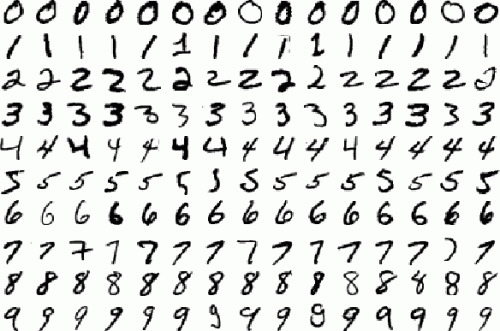
\includegraphics[width=90mm]{./images/mnistdigits.jpg}
\caption{Example MNIST digit images \label{overflow}}
\end{figure}


For this example, we will download and import the train and test datasets from a public Amazon S3 bucket.%: {\url{https://h2o-public-test-data.s3.amazonaws.com/smalldata/testng/higgs_train_5k.csv}}
The train file is 13MB and the test file is 2.1MB, and below we download the data directly so the speed that the data is imported is limited by download speed.  Files can be uploaded from a variety of sources, including a remote locations and HDFS.

\newpage
\waterExampleInR
%Load the data to your current working directory in your R Console (do this for any future dataset downloads), and then run the following command.
\lstinputlisting[style=R]{deeplearning/deeplearning_importfile_example.R}

\waterExampleInPython
\lstinputlisting[style=python]{deeplearning/deeplearning_importfile_example.py}

\subsection{Performing a trial run}
\label{ssec:TrialRun} 
The example below illustrates the relative simplicity underlying most H2O Deep Learning model parameter configurations, as a result of the default settings. We use the first $28^2 = 784$ values of each row to represent the full image and the final value to denote the digit class. Rectified linear activation is popular with image processing and has performed well on the MNIST database previously and dropout has been known to enhance performance on this dataset as well, so we train our model accordingly. 

% Old R example:
%\begin{lstlisting}[style=R]
%#Train the model for digit classification
%mnist_model = h2o.deeplearning(x = 1:784, y = 785, data = train_images.hex, activation = "RectifierWithDropout", hidden = c(200,200,200), input_dropout_ratio = 0.2, l1 = 1e-5, validation = test_images.hex, epochs = 10)
%
%\end{lstlisting}
%\normalsize

\waterExampleInR
\lstinputlisting[style=R]{deeplearning/deeplearning_examplerun.R}

% TO DO: Add this code (currently commented out)
\waterExampleInPython
\lstinputlisting[style=python]{deeplearning/deeplearning_examplerun.py}


\noindent
The model runs for only 10 epochs since it is just meant  as a trial run. In this trial run, we also specified the validation set as the test set.  In addition to, or instead of using a validation set, another option is to use k-fold validation by specifying, for example, \texttt{nfolds = 5} in addition to / instead of \texttt{validation\_frame = test}.  When \texttt{nfolds} is a positive integer, k-fold cross validation will be performed and the cross-validation metrics will be computed.  Optionally, the user can save the cross-validation predicted values (generated during cross-validation) by setting \texttt{keep\_cross\_validation\_predictions} parameter to true.  

\subsubsection{Extracting and handling the results} 

We can extract the parameters of our model, examine the scoring process, and make predictions on new data.

\waterExampleInR
\lstinputlisting[style=R]{deeplearning/deeplearning_inspect_model.R}

% TO DO: Add this code (currently commented out)
\waterExampleInPython
\lstinputlisting[style=python]{deeplearning/deeplearning_inspect_model.py}



\noindent
The second command returns the training and validation errors for the model. The training error value is based on the parameter \texttt{score\_training\_samples}, which specifies the number of randomly sampled training points to be used for scoring (the default uses 10,000 points). The validation error is based on the parameter \texttt{score\_validation\_samples}, which configures the same value on the validation set; by default, this is the entire validation set.

In general, choosing a greater number of sampled points leads to a better understanding of the model's performance on your dataset; setting either of these parameters to 0 automatically uses the entire corresponding dataset for scoring. However, either method allows you to control the minimum and maximum time spent on scoring with the \texttt{score\_interval} and \texttt{score\_duty\_cycle} parameters.
\\
\\
These scoring parameters also affect the final model when the parameter \texttt{overwrite\_with\_best\_model} is enabled. This option selects the model that achieved the lowest validation error during training (based on the sampled points used for scoring) as the final model after training. If a dataset is not specified as the validation set, the training data is used by default; in this case, either the \texttt{score\_training\_samples} or \texttt{score\_validation\_samples} parameter will control the error computation during training and, in turn, the selected best model.
\\
\\
Once we have a satisfactory model, the \texttt{h2o.predict()} command can be used to compute and store predictions on new data, which can then be used for further tasks in the interactive data science process.

\waterExampleInR
\lstinputlisting[style=R]{deeplearning/deeplearning_predict.R}

\waterExampleInPython
\lstinputlisting[style=python]{deeplearning/deeplearning_predict.py}



\subsection{Web interface} 

H2O R users have access to an intuitive web interface for H2O, Flow, to mirror the model building process in R. After loading data or training a model in R, point your browser to your IP address and port number (e.g., localhost:12345) to launch the web interface. From here, you can click on \textsc{Admin} $>$ \textsc{Jobs} to view specific details about your model. You can also click on \textsc{Data} $>$ \textsc{List All Frames} to view all current H2O frames. 

\subsubsection{Variable importances} 

The variable importances feature can be enabled with the argument \texttt{variable\_importances = TRUE}. This feature allows us to view the absolute and relative predictive strength of each feature in the prediction task.  Each H2O algorithm class has it's own methodology for computing variable importance.  For H2O's Deep Learning, the Gedeon method is used, which can be slow for large networks, so it is turned off by default.  If variable importance is the top priority in your analysis, you may (also) consider training a Random Forest and inspecting the variable importances generated with that method.

The following code demonstrates training using the \texttt{variable\_importances} option enabled and how to extract the variable importances from the trained model.  From the web UI, you can also view a visualization of the variable importances.

\waterExampleInR
\lstinputlisting[style=R]{deeplearning/deeplearning_varimp.R}

%\medskip
\waterExampleInPython
\lstinputlisting[style=python]{deeplearning/deeplearning_varimp.py}



\subsubsection{Java model} 

Another important feature of the web interface is the Java (POJO) model, accessible from the \textsc{Preview POJO} button at the bottom of the model results. This button allows access to Java code that builds the model when called from a main method in a Java program. Instructions for downloading and running this Java code are available from the web interface, and example production scoring code is available as well.

\subsection{Grid search for model comparison} 

H2O supports grid search capabilities for model tuning by allowing users to tweak certain parameters and observe changes in model behavior. This is done by specifying sets of values for parameter arguments. The following example represents a sample grid search:

%\begin{lstlisting}[style=R]
%#Create a set of network topologies
%hidden_layers = list(c(200,200), c(100,300,100),c(500,500,500))
%
%mnist_model_grid = h2o.deeplearning(x = 1:784, y = 785, data = train_images.hex, activation = "RectifierWithDropout", hidden = hidden_layers, validation = test_images.hex, epochs = 1, l1 = c(1e-5,1e-7), input_dropout_ratio = 0.2)
%
%\end{lstlisting}

\waterExampleInR
\lstinputlisting[style=R]{deeplearning/deeplearning_gridsearch.R}

%\medskip
\waterExampleInPython
\lstinputlisting[style=python]{deeplearning/deeplearning_gridsearch.py}


\normalsize
\noindent
In this example, we specified three different network topologies and two different $\ell_1$ norm weights. This grid search model trains six different models using all possible combinations of these parameters; other parameter combinations can be specified for a larger space of models. This provides more subtle insights into the model tuning and selection process by inspecting and comparing our trained models after the grid search process is complete. To learn how and when to select different parameter configurations in a grid search, refer to Appendix A for parameter descriptions and configurable values.

%\begin{lstlisting}[style=R]
%#print out all prediction errors and run times of the models
%mnist_model_grid
%mnist_model_grid@model
%
%#print out a *short* summary of each of the models (indexed by parameter)
%mnist_model_grid@sumtable
%
%#print out *full* summary of each of the models
%all_params = lapply(mnist_model_grid@model, function(x) { x@model$params })
%all_params
%
%#access a particular parameter across all models
%l1_params = lapply(mnist_model_grid@model, function(x) { x@model$params$l1 })
%l1_params
%\end{lstlisting}

\waterExampleInR
\lstinputlisting[style=R]{deeplearning/deeplearning_gridsearch_result.R}

%\medskip
\waterExampleInPython
\lstinputlisting[style=python]{deeplearning/deeplearning_gridsearch_result.py}


% HERE (Have not edited the rest of Ch 6  - 7; Appendix has been edited though)
\subsection{Checkpoint model}

To resume model training, use checkpoint model keys for incrementally training a particular model with more iterations, more data, different data, and so forth. To train our initial model further, we can use it (or its key) as a checkpoint argument for a new model.

In the command below, \texttt{mnist\_model\_grid@model[[1]]} represents the highest performing model from the grid search used for additional training. For checkpoint restarts, the training and validation datasets, as well as the response column, must match.

\begin{lstlisting}[style=R]
mnist_checkpoint_model = h2o.deeplearning(x=1:784, y=785, data=train_images.hex, checkpoint=mnist_model_grid@model[[1]], validation = test_images.hex, epochs=9)

\end{lstlisting}
\noindent
Checkpointing can also be used to reload existing models that were saved to disk in a previous session. For example, we can save and reload the best model from the grid search by running the following commands.

\begin{lstlisting}[style=R]
#Specify a model and the file path where it is to be saved
h2o.saveModel(object = mnist_model_grid@model[[1]], name = "/tmp/mymodel", force = TRUE)

#Alternatively, save the model key in some directory (here we use /tmp)
#h2o.saveModel(object = mnist_model_grid@model[[1]], dir = "/tmp", force = TRUE)

\end{lstlisting}
\normalsize

\noindent
After restarting  H2O, load the saved model by specifying the host and saved model file path. \textbf{Note}: The saved model must be reloaded using a compatible H2O version (i.e., the same version used to save the model).

\begin{lstlisting}[style=R]
best_mnist_grid.load = h2o.loadModel(h2o_server, "/tmp/mymodel")

#Continue training the loaded model
best_mnist_grid.continue = h2o.deeplearning(x=1:784, y=785, data=train_images.hex, checkpoint=best_mnist_grid.load, validation = test_images.hex, epochs=1)

\end{lstlisting}
\normalsize

\noindent
Additionally, you can also use the command
\begin{lstlisting}[style=R]
model = h2o.getModel(h2o_server, key)

\end{lstlisting}
\noindent
to retrieve a model from its H2O key. This command is useful, for example, if you have created an H2O model using the web interface and wish to proceed with the modeling process in R.

\subsection{Achieving world-record performance}

Without distortions, convolutions, or other advanced image processing techniques, the best-ever published test set error for the MNIST dataset is $0.83$\% by Microsoft. After training for $2,000$ epochs (took about 4 hours) on 4 compute nodes, we obtain $0.87\%$ test set error and after training for $8,000$ epochs (took about 10 hours) on 10 nodes, we obtain $0.83\%$ test set error, which is the current world-record, notably achieved using a distributed configuration and with a simple 1-liner from R. Details can be found in our \href{http://learn.h2o.ai/content/hands-on_training/deep_learning.html}{hands-on tutorial}. Accuracies around $1\%$ test set errors are typically achieved within 1 hour when running on 1 node.
The parallel scalability of H2O for the MNIST dataset on 1 to 63 compute nodes is shown in the figure below.
\begin{figure}[h!]
\centering
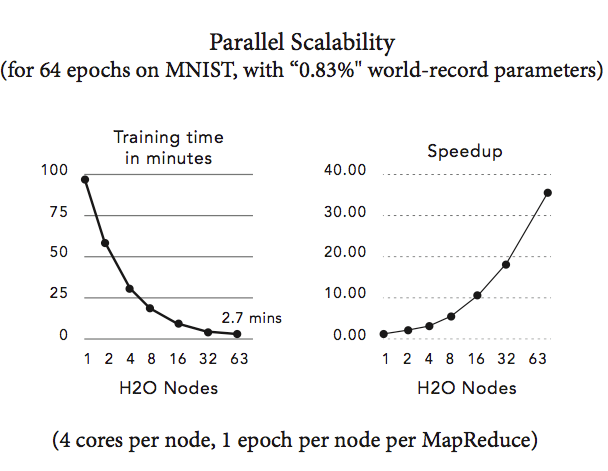
\includegraphics{scalability_new.png}
\end{figure}
\bigskip
\bigskip
\bigskip
\section{Deep Autoencoders}
\label{sec:DeepAutoencoders}  

\subsection{Nonlinear dimensionality reduction} 
So far, we have discussed purely supervised deep learning tasks. However, deep learning can also be used for unsupervised feature learning or, more specifically, nonlinear dimensionality reduction  (\href{http://www.cs.toronto.edu/~hinton/science.pdf}{Hinton et al, 2006}). Consider the diagram of a three-layer neural network with one hidden layer on the following page. If we treat our input data as labeled with the same input values, then the network is forced to learn the identity via a nonlinear, reduced representation of the original data. This type of algorithm is called a deep autoencoder; these models have been used extensively for unsupervised, layer-wise pre-training of supervised deep learning tasks, but here we discuss the autoencoder's ability to discover anomalies in data. 
\\
\begin{figure}[h!]
\centering
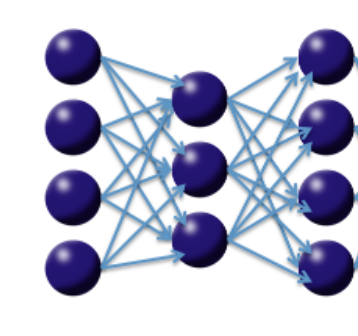
\includegraphics[scale=0.7]{autoencoder.png}
\end{figure}
\subsection{Use case: anomaly detection} %%TODO: do we still want to use this example?
Consider the deep autoencoder model described above. Given enough training data that resembles some underlying pattern, the network will train itself to easily learn the identity when confronted with that pattern. However, if some ``anomalous" test point that does not match the learned pattern arrives, the autoencoder will likely have a high error in reconstructing this data, which indicates it is anomalous data.
\\
\\
We use this framework to develop an anomaly detection demonstration using a deep autoencoder. The dataset is an ECG time series of heartbeats and the goal is to determine which heartbeats are outliers. The training data (20 ``good" heartbeats) and the test data (training data with 3 ``bad" heartbeats appended for simplicity) can be downloaded from the H2O GitHub repository for the H2O Deep Learning documentation at http://bit.ly/1yywZzi%%update.%% 
Each row represents a single heartbeat. The autoencoder is trained as follows: 

\begin{lstlisting}[style=R]
train_ecg.hex = h2o.uploadFile(h2o_server, path="ecg_train.csv", header=F, sep=",", key="train_ecg.hex") 
test_ecg.hex = h2o.uploadFile(h2o_server, path="ecg_test.csv", header=F, sep=",", key="test_ecg.hex") 

#Train deep autoencoder learning model on "normal" training data, y ignored 
anomaly_model = h2o.deeplearning(x=1:210, y=1, train_ecg.hex, activation = "Tanh", classification=F, autoencoder=T, hidden = c(50,20,50), l1=1E-4, 
epochs=100)                 
                              
#Compute reconstruction error with the Anomaly detection app (MSE between output layer and input layer)
recon_error.hex = h2o.anomaly(test_ecg.hex, anomaly_model)
                              
#Pull reconstruction error data into R and plot to find outliers (last 3 heartbeats)
recon_error = as.data.frame(recon_error.hex)
recon_error
plot.ts(recon_error)

#Note: Testing = Reconstructing the test dataset
test_recon.hex = h2o.predict(anomaly_model, test_ecg.hex) 
head(test_recon.hex)              

\end{lstlisting}
\noindent

\newpage

\section{Appendix A: Complete parameter list}
\begin{itemize}

\item \texttt{x}: A vector containing the names of the predictors in the model. No default.

\item \texttt{y}: The name of the response variable in the model. No default.

\item \texttt{training\_frame}: An \texttt{H2OFrame} object containing the variables in the model.  No default.

\item \texttt{model\_id}: (Optional) The unique ID assigned to the resulting model. If not specified, an ID is generated automatically. 

\item \texttt{overwrite\_with\_best\_model}: Logical. If enabled, overwrite the final model with the best model found during training. Default is true.

\item \texttt{validation\_frame}: (Optional) An \texttt{H2OFrame} object that represents the validation dataset used to construct the confusion matrix. If blank and \texttt{nfolds = 0}, the training data is used by default. 

\item \texttt{checkpoint}: (Optional) Model checkpoint (either key or H2ODeepLearningModel) used to resume training. 

\item \texttt{autoencoder}: Logical. Enable autoencoder; default is false. Refer to the ``\nameref{sec:DeepAutoencoders}'' section for more details.

\item \texttt{use\_all\_factor\_levels}: Logical. Use all factor levels of categorical variance. Otherwise, the first factor level is omitted (without loss of accuracy). Useful for variable importances and auto-enabled for autoencoder.  Default is true.

\item \texttt{activation}: The choice of nonlinear, differentiable activation function used throughout the network. Options are \texttt{Tanh, TanhWithDropout, Rectifier, RectifierWithDropout, Maxout, MaxoutWithDropout}, and the default is \texttt{Rectifier}. Refer to the ``\nameref{sssec:ActivationLoss}'' section for more details.

\item \texttt{hidden}: The number and size of each hidden layer in the model. For example, if \texttt{c(100,200,100)} is specified, a model with 3 hidden layers will be produced, the middle hidden layer will have 200 neurons and the first and third hidden layers will have 100 neurons. The default is \texttt{c(200,200)}. For grid search, use \texttt{list(c(10,10), c(20,20))} etc. Refer to the section on  ``\nameref{ssec:TrialRun}'' for more details. 

\item \texttt{epochs}: The number of passes or over the training dataset (can be fractional). It is recommended to start with lower values for initial grid searches. The value can be modified during checkpoint restarts and allows continuation of selected models. Default is 10.

\item \texttt{train\_samples\_per\_iteration}: The number of training samples (globally) per MapReduce iteration. The following special values are also supported: \texttt{0} (one epoch); \texttt{-1} (all available data; e.g., replicated training data); \texttt{-2} (auto-tuning; default). Refer to the ``\nameref{sssec:TrainSamplesPerIter}'' for more details.
%HERE
\item \texttt{seed}: The random seed controls sampling and initialization. Reproducible results are only expected with single-threaded operation (i.e. when running on one node, turning off load balancing and providing a small dataset that fits in one chunk).  In general, the multi-threaded asynchronous updates to the model parameters will result in (intentional) race conditions and non-reproducible results.  Default is a randomly generated number.

\item \texttt{adaptive\_rate}: Logical.  Enables adaptive learning rate (ADADELTA). Default is true. Refer to the ``\nameref{sssec:AdaptiveLearning}'' section for more details.

\item \texttt{rho}: Adaptive learning rate time decay factor. This parameter is similar to momentum and relates to the memory to prior weight updates. Typical values are between 0.9 and 0.999. Default value is 0.99. %The value of \texttt{rho} must be greater than zero if \texttt{epsilon} is greater than zero. 
Refer to the section on ``\nameref{sssec:AdaptiveLearning}'' for more details. 

\item \texttt{epsilon}: The second of two hyperparameters for adaptive learning rate (when it is enabled). This parameter is similar to learning rate annealing during initial training and momentum at later stages where it allows forward progress. Typical values are between 1e-10 and 1e-4. This parameter is only active if \texttt{adaptive\_rate} is enabled. Default is 1e-8. %The value of \texttt{epsilon} must be greater than zero if \texttt{rho} is greater than zero.   
Refer to the ``\nameref{sssec:AdaptiveLearning}'' section for more details.

\item \texttt{rate}: The learning rate, $\alpha$. Higher values lead to less stable models, while lower values lead to slower convergence. Default is 0.005.  %%is this still supported? 

\item \texttt{rate\_annealing}: The annealing learning rate is calculated as \texttt{(rate)}/(1+\texttt{rate\_annealing} * N), where N is the number of training samples.  It is the inverse of the number of training samples required to cut the learning rate in half.  This reduces the learning rate to ``freeze'' into local minima in the optimization landscape.  Default value is 1e-6 (when adaptive learning is disabled). Refer to the ``\nameref{sssec:RateAnnealing}'' section for more details.

\item \texttt{rate\_decay}: Learning rate decay factor between layers (L-th layer: \texttt{rate} * \texttt{rate\_decay\^} (L-1)); default is 1.0 (when adaptive learning is disabled). The learning rate decay parameter controls the change of learning rate across layers.

\item \texttt{momentum\_start}: This controls the amount of momentum at the beginning of training (when adaptive learning is disabled). Default is 0. Refer to the ``\nameref{sssec:MomentumTraining}'' section for more details.

\item \texttt{momentum\_ramp}: This controls the amount of learning for which momentum increases (assuming \texttt{momentum\_stable} is larger than \texttt{momentum\_start}).  The ramp is measured in the number of training samples and can be enabled when adaptive learning is disabled. Default is 1 million (1e6). Refer to the  ``\nameref{sssec:MomentumTraining}'' section or more details.

\item \texttt{momentum\_stable}: This controls the final momentum value reached after \texttt{momentum\_ramp} number of training samples (when adaptive learning is disabled). The momentum used for training will remain the same for training beyond reaching that point. Default is 0.  Refer to the ``\nameref{sssec:MomentumTraining}'' for more details.

\item \texttt{nesterov\_accelerated\_gradient}:  Logical.  The Nesterov accelerated gradient descent method is a modification to traditional gradient descent for convex functions. The method relies on gradient information at various points to build a polynomial approximation that minimizes the residuals in fewer iterations of the descent. This parameter is only active if adaptive learning rate is disabled.  The default is true (when adaptive learning is disabled). Refer to the ``\nameref{sssec:MomentumTraining}'' section for more details.

\item \texttt{input\_dropout\_ratio}: The fraction of the features for each training row to be omitted from training in order to improve generalization. The default is 0 (always use all features).  Refer to the ``\nameref{ssec:Regularization}'' section for more details.

\item \texttt{hidden\_dropout\_ratios}:  The fraction of the inputs for each hidden layer to be omitted from training in order to improve generalization. The default is 0.5 for each hidden layer.  Refer to the ``\nameref{ssec:Regularization}'' section for more details.

\item \texttt{l1}: L1 regularization, which constrains the absolute value of the weights (can add stability and improve generalization, causes many weights to become 0). The default is 0, for no L1 regularization. Refer to the ``\nameref{ssec:Regularization}'' section for more details.

\item \texttt{l2}: L2 regularization, which constrains the sum of the squared weights (can add stability and improve generalization, causes many weights to be small). The default is 0, for no L2 regularization. Refer to the ``\nameref{ssec:Regularization}'' section for more details.

\item \texttt{max\_w2}: A maximum on the sum of the squared incoming weights into any one neuron. This tuning parameter is especially useful for unbound activation functions such as Maxout or Rectifier. The default, positive infinity, leaves this maximum unbounded.

\item \texttt{initial\_weight\_distribution}: The distribution from which initial weights are to be drawn. Select \texttt{Uniform, UniformAdaptive} or \texttt{Normal}. Default is \texttt{UniformAdaptive}. Refer to the ``\nameref{sssec:Initialization}'' for more details.

\item \texttt{initial\_weight\_scale}: The scale of the distribution function for Uniform or Normal distributions. For Uniform, the values are drawn uniformly from (-\texttt{initial\_weight\_scale, initial\_weight\_scale}). For Normal, the values are drawn from a Normal distribution with a standard deviation of \texttt{initial\_weight\_scale}. The default is 1. Refer to the ``\nameref{sssec:Initialization}'' for more details.

\item \texttt{loss}: Specify one of the loss options: \texttt{Automatic, CrossEntropy} (for classification only), \texttt{MeanSquare, Absolute}, or \texttt{Huber}. Refer to the ``\nameref{sssec:ActivationLoss}'' section for more details.

\item \texttt{distribution}: Specify the distribution function of the response: \texttt{AUTO, bernouilli, multinomial, poisson, gamma, tweedie, laplace, huber,} or \texttt{gaussian}. 

\item \texttt{tweedie\_power}: Specify the tweedie power; applicable only if \texttt{distribution} is set to \texttt{tweedie}. Value must be between 1.0 and 2.0. 

\item \texttt{score\_interval}: The minimum time (in seconds) to elapse between model scoring. The actual interval is determined by the number of training samples per iteration and the scoring duty cycle. To use all training set samples, specify \texttt{0}. Default is 5.

\item \texttt{score\_training\_samples}: The number of training samples to be used for scoring.  These samples will be randomly sampled. Use 0 to select the entire training dataset.  Default is 10000.

\item \texttt{score\_validation\_samples}: The number of validation dataset points to be used for scoring. Can be randomly sampled or stratified (if  \texttt{balance\_classes} is set and \texttt{score\_validation\_sampling} is set to stratify). Use 0 to select the entire validation dataset (default).

\item \texttt{score\_duty\_cycle}: Maximum duty cycle fraction spent on model scoring (on both training and validation samples), and on diagnostics such as computation of feature importances (i.e., not on training). Lower values result in more training, while higher values produce more scoring. Default is 0.1.

\item \texttt{classification\_stop}: The stopping criterion for classification error (1 - accuracy) on the training data scoring dataset.  When the error is at or below this threshold, the training process stops.  Default is 0.  To disable, enter \texttt{-1}. 

\item \texttt{regression\_stop}: The stopping criterion for regression error (MSE) on the training data scoring dataset. When the error is at or below this threshold, the training process stops. Default is 1e-6.  To disable, enter \texttt{-1}. 

\item \texttt{quiet\_mode}: Logical. Enable quiet mode for less output to standard output. Default is false.

\item \texttt{max\_confusion\_matrix\_size}: For classification models, the maximum size (in terms of classes) of the confusion matrix to display. This option is meant to avoid printing extremely large confusion matrices. Default is 20.

\item \texttt{max\_hit\_ratio\_k}: The maximum number (top K) of predictions to use for hit ratio computation (for multi-class only, enter 0 to disable). Default is 10.

\item \texttt{balance\_classes}: Logical. For imbalanced data, the training data class counts can be artificially balanced by over-sampling the minority class(es) and under-sampling the majority class(es) so that each class will contain the same number of observations.  This can result in improved predictive accuracy.  Over-sampling is done with replacement (rather than simulating new observations), and the total number of observations after balancing is controlled by the \texttt{max\_after\_balance\_size} parameter.  Default is false.
%This means that the maximum number of obs will be 5*N, where N is the number of observations in the original (unbalanced) training set.  If you want the balanced training set to have the same number of obs as the original training set, then set this to argument to 1.  

\item \texttt{class\_sampling\_factors}: Desired over/under-sampling ratios per class (in lexicographic order). Only applies to classification when \texttt{balance\_classes} is enabled. If not specified, the ratios will be automatically computed to obtain class balance during training.

\item \texttt{max\_after\_balance\_size}: When classes are balanced, limit the resulting dataset size to the specified multiple of the original dataset size. This is the maximum relative size of the training data after balancing class counts (can be less than 1.0). Default is 5.

\item \texttt{score\_validation\_sampling}: Method used to sample validation dataset for scoring. The possible methods are \texttt{Uniform} and \texttt{Stratified}. Default is \texttt{Uniform}.

\item \texttt{diagnostics}: (Deprecated) Logical. Gather diagnostics for hidden layers, such as mean and root mean squared (RMS) values of learning rate, momentum, weights and biases. Since deprecation, diagnostics are always enabled (set to true).

\item \texttt{variable\_importances}: Logical. Compute variable importances for input features using the Gedeon method. The implementation considers the weights connecting the input features to the first two hidden layers. Default is false, since this can be slow for large networks. 

\item \texttt{fast\_mode}: Logical. Enable fast mode (minor approximation in back-propagation).  This should not affect results significantly. Default is true.

\item \texttt{ignore\_const\_cols}: Logical. Ignore constant training columns (no information can be gained anyway). Default is true.

\item \texttt{force\_load\_balance}:  Logical. Force extra load balancing to increase training speed for small datasets to keep all cores busy. Default is true.

\item \texttt{replicate\_training\_data}:  Logical. Replicate the entire training dataset onto every node for faster training on small datasets. Default is true.

\item \texttt{single\_node\_mode}:  Logical. Run on a single node for fine-tuning of model parameters. Can be useful for faster convergence during checkpoint resumes after training on a very large count of nodes (for fast initial convergence). Default is false.

\item \texttt{shuffle\_training\_data}: Logical.  Enable shuffling of training data (on each node). This option is recommended if training data is replicated on N nodes, and the number of training samples per iteration is close to N times the dataset size, where all nodes train with (almost) all of the data. It is automatically enabled if the number of training samples per iteration is set to -1 (or to N times the dataset size or larger).  Default is false.

\item \texttt{sparse}: (Deprecated) Logical. Enable sparse data handling.% (Experimental). 
Default is false.

\item \texttt{col\_major}: (Deprecated) Logical. Use a column major weight matrix for the input layer; can speed up forward propagation, but may slow down backpropagation. Default is false.

\item \texttt{average\_activation}: Specify the average activation for the sparse autoencoder (Experimental).
Default is 0.

\item \texttt{sparsity\_beta}: Specify the sparsity-based regularization optimization (Experimental).  Default is 0. 

\item \texttt{max\_categorical\_features}:  Maximum number of categorical features allowed in a column, enforced via hashing (Experimental).  Default is $2^{31}-1$ (\texttt{Integer.MAX\_VALUE} in Java).

\item \texttt{reproducible}: Logical. Force reproducibility on small data (will be slow -- only uses one thread).  Default is false.

\item \texttt{export\_weights\_and\_biases}: Logical. Specify whether to export the neural network weights and biases as an \texttt{H2OFrame}.  Default is false.

% TO DO: Should these be added?  They are in the Java code, but not documented elsewhere
%  public boolean _elastic_averaging = false;
%  public double _elastic_averaging_moving_rate = 0.9;
%  public double _elastic_averaging_regularization = 1e-3;
%
%  // stochastic gradient descent: mini-batch size = 1
%  // batch gradient descent: mini-batch size = # training rows
%  public int _mini_batch_size = 1;

\item \texttt{offset\_column}:  Specify the offset column by column name.  Regression only.  Offsets are per-row ``bias values''�� that are used during model training. For Gaussian distributions, they can be seen as simple corrections to the response (y) column. Instead of learning to predict the response value directly, the model learns to predict the (row) offset of the response column. For other distributions, the offset corrections are applied in the linearized space before applying the inverse link function to get the actual response values. 

\item \texttt{weights\_column}: Specify the weights column by column name. Weights are per-row observation weights. This is typically the number of times a row is repeated, but non-integer values are supported as well. During training, rows with higher weights matter more, due to the larger loss function pre-factor.

\item \texttt{nfolds}: (Optional) Number of folds for cross-validation. % If the number of folds is greater than or equal to 2, then validation must remain empty. 
Default is 0 (no cross-validation is performed).

\item \texttt{fold\_column}: (Optional) Name of column with cross-validation fold index assignment per observation; the folds are supplied by the user. 

\item \texttt{fold\_assignment}: Cross-validation fold assignment scheme, if \texttt{nfolds} is greater than zero and \texttt{fold\_column} is not specified. Options are \texttt{AUTO, Random,} or \texttt{Modulo}. 

\item \texttt{keep\_cross\_validation\_predictions}: Logical.  Specify whether to keep the predictions of the cross-validation models.  Default is false.

\end{itemize}


\newpage
\section{Appendix B: References}

\textbf{H2O website}:  {\url{http://h2o.ai/}}

\textbf{H2O documentation}:  {\url{http://docs.h2o.ai}}

\textbf{H2O Github Repository}:  {\url{http://github.com/h2oai/h2o.git}}

\textbf{H2O Training}:    {\url{http://learn.h2o.ai/}}

\textbf{H2O Training Scripts and Data}: {\url{http://data.h2o.ai/}} 

\textbf{Code for this Document}:   \\
 {\url{https://github.com/h2oai/h2o/tree/master/docs/deeplearning/DeepLearningRVignetteDemo}}

\textbf{H2O support}:   {\url{h2ostream@googlegroups.com}}

\textbf{H2O JIRA}: {\url{https://0xdata.atlassian.net/secure/Dashboard.jspa}}

\textbf{YouTube Channel}: {\url{https://www.youtube.com/user/0xdata}}

\textbf{Learning Deep Architectures for AI}. Bengio, Yoshua, 2009. \\
 {\url{http://www.iro.umontreal.ca/~lisa/pointeurs/TR1312.pdf}}

\textbf{Efficient BackProp}.  {LeCun et al, 1998}. {\url{http://yann.lecun.com/exdb/publis/pdf/lecun-98b.pdf}}

\textbf{Maxout Networks}. {Goodfellow et al, 2013}.  {\url{http://arxiv.org/pdf/1302.4389.pdf}}

\textbf{HOGWILD!: A Lock-Free Approach to Parallelizing Stochastic Gradient Descent}.  \\
{Niu et al, 2011}.  {\url{http://i.stanford.edu/hazy/papers/hogwild-nips.pdf}}

\textbf{Improving neural networks by preventing co-adaptation of feature detectors}.  \\
{Hinton et al., 2012}.  \href{http://arxiv.org/pdf/1207.0580.pdf}{http://arxiv.org/pdf/1207.0580.pdf}

\textbf{On the importance of initialization and momentum in deep learning}.  {Sutskever et al, 2014}.  \href{http://www.cs.toronto.edu/~fritz/absps/momentum.pdf}{http://www.cs.toronto.edu/~fritz/absps/momentum.pdf}

\textbf{ADADELTA: An Adaptive Learning Rate Method}. {Zeiler, 2012}.  \\
 \href{http://arxiv.org/pdf/1212.5701v1.pdf}{http://arxiv.org/pdf/1212.5701v1.pdf}

\textbf{H2O GitHub repository for the H2O Deep Learning documentation} \\
 \href{https://github.com/h2oai/h2o/tree/master/docs/deeplearning/DeepLearningRVignetteDemo}{https://github.com/h2oai/h2o/tree/master/docs/deeplearning/DeepLearningRVignetteDemo}

\textbf{{MNIST database.}}  \href{http://yann.lecun.com/exdb/mnist/}{http://yann.lecun.com/exdb/mnist/}

\textbf{Reducing the Dimensionality of
Data with Neural Networks}.  {Hinton et al, 2006}. \\
 \href{http://www.cs.toronto.edu/~hinton/science.pdf}{http://www.cs.toronto.edu/~hinton/science.pdf}

\textbf{Definitive Performance Tuning Guide for Deep Learning}. \href{http://h2o.ai/blog/2015/02/deep-learning-performance/}{http://h2o.ai/blog/2015/02/deep-learning-performance/}

%%TODO: add Arno's performance guide blog post after it is updated; need a good way to include bar charts for results - can re-create in Photoshop if needed, but we should definitely include a link to the script

%%TODO: Remove `maxout` refs, add "mini-badge" parameter?


\end{document}
